\begin{song}{title=\predtitle\centering Ve skříni \\\large Karel Plíhal \vspace*{-0.3cm}}  %% sem se napíše jméno songu a autor

\moveright -1cm \vbox{

\begin{centerjustified}
\nejnejvetsi

\begin{varwidth}[t]{0.55\textwidth}\setlength{\parindent}{\pindent}  %Varianta č. 2 --> Dva sloupce

\sloka
^{A\z}Kdesi ^{D\z}dole v ^{D\z}babiččině ^{A\z}skříni

bydlí ^{\z D}beduíni, ^{G}v ^{\z Cmi}její ^{A\z}skříni.

Křičí ^{D}na mě, kámo dej mi ^{A\z}čouda,

^{A\z}cígo za ^{D}velblouda, ^{G\,\,Emi}křičí ^{A}na ^{D}mě.


\refren
^{D\z}Dlouhý ^{G\z}karavany

^{D\z}jdou hlavní ^{A\z D}třídou,

^{D\z}dlouhý ^{G\z}karavany ^{D\z}jdou, já ^*{A\,}jdu~s~nim a

^{D\z}zapít ^{G\z}trable, který ^{D\,\,}jsou, který ^{A\z D}přijdou,

^{D}je to ^{G\z}príma chvíli ^{Hmi\z}být~mezi ^{A\z G}svýma.

\end{varwidth}\mezisloupci\begin{varwidth}[t]{0.55\textwidth}\setlength{\parindent}{\pindent}\vspace*{0.55cm}  % V případě varianty č.2 jde odsud text do pravé části

\sloka
Člověk míní, Pan Bůh zase mění,

beduíni v skříni zabydlení

hrají karty, pijí vodu z misek,

kdy je Šrámkův Písek vyzvídají.

\ssloka{(\textbf{R:})}

\mezera

V šeru skříně tiše dřepí blázen,

touží po oáze, po tvém klíně.

\end{varwidth}
\end{centerjustified}
}

\centering
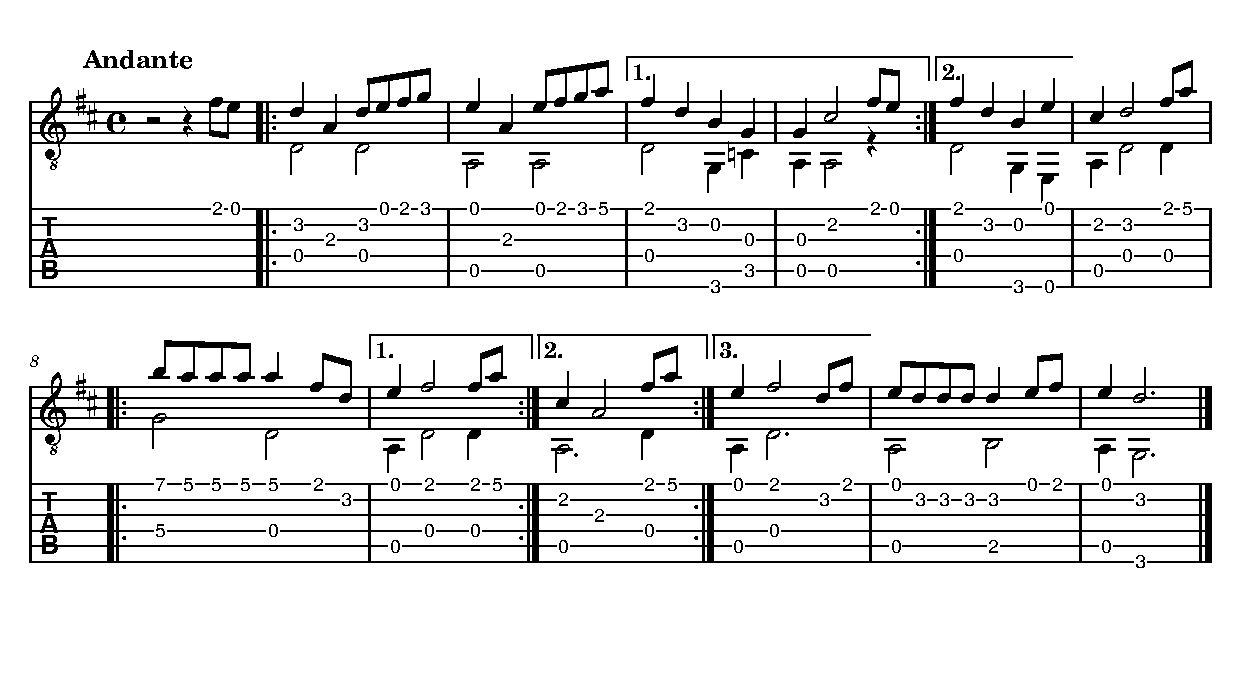
\includegraphics[scale=\defaulttabscale]{../taby/veskrini.pdf}

\setcounter{Slokočet}{0}
\end{song}
